\chapter{Optimization and Neural Networks}
\label{ch:optimization-neural-networks}

Chapter~\ref{ch:structure-beyond-linearity} broadened the idea of structure by adding branches, margins, neighborhoods, and unsupervised organization. Neural networks take a different step. Instead of asking only which rule to place on top of a representation, they allow part of the representation itself to be learned from data. That added flexibility is useful only when it is disciplined by optimization, regularization, and careful evaluation.

This chapter explains that learning process without mystifying it. It moves from learned feature pipelines to forward passes, losses, optimization, debugging, and generalization, and it ends with a minimum credible neural training report. The goal is not only to show how neural networks work, but to show what evidence makes a neural result worth trusting.

\section{Opening Dilemma: When Engineered Structure Stops Being Enough}

The earlier modeling chapters already established a core logic. We frame a task, design an evaluation plan, try a serious baseline, and inspect what kind of structure that baseline is missing. Sometimes the answer is still manageable with trees, engineered interactions, or geometry-based methods. Sometimes it is not.

Images, language, and audio often contain structure that is difficult to specify manually at the right level of abstraction. Even in smaller problems, the useful intermediate signals may not be obvious in advance. In such cases, the main challenge is not only drawing the final decision boundary. It is discovering the space in which that boundary should be drawn.

That is when learned structure becomes the right move. The issue is not merely that deep learning is powerful. The issue is that the representation itself is part of what must be learned.

This does not mean neural networks are always the best choice. On small tabular datasets, a linear model or tree ensemble may still be stronger, easier to debug, and easier to justify. The important shift is conceptual: neural networks are most valuable when the main modeling problem is that the useful internal features are unknown.

The practical workflow is equally simple to state in prose. Start with the strongest simple baseline, decide what structure it is missing, build the smallest network that could plausibly learn that structure, train with a validation split while watching for optimization versus generalization failure, and then report the result in a minimum credible training report.

Chapter~\ref{ch:structure-beyond-linearity} asked which kind of structure should be added next. This chapter asks what happens when the structure itself is not fully specified in advance and must instead be learned during training.

\section{A Neural Network as a Learned Feature Pipeline}

\begin{practicalnote}
\textbf{Terminology shift.} In earlier chapters, ``features'' meant attributes designed by the practitioner---one-hot encodings, polynomial terms, bag-of-words counts. From this chapter onward, ``features'' will also refer to the \emph{learned} intermediate representations that a neural network discovers during training. Where the distinction matters, this chapter says ``hand-designed features'' for the earlier sense and ``learned features'' or ``internal features'' for the new one.
\end{practicalnote}

The conceptual heart of the chapter is simple:

\begin{center}
\emph{raw input $\rightarrow$ learned intermediate features $\rightarrow$ final score or probability}
\end{center}

A hidden layer is not extra decoration. It is a learned representation stage. Everything else in the chapter explains how that pipeline is computed, corrected, stabilized, and judged.

\begin{figure}[t]
\centering
\definecolor{c6mlBg}{RGB}{220,233,251}
\definecolor{c6mlLine}{RGB}{56,103,170}
\definecolor{c6nnBg}{RGB}{210,238,220}
\definecolor{c6nnLine}{RGB}{26,112,64}
\resizebox{\linewidth}{!}{%
\begin{tikzpicture}[x=1cm, y=1cm, font=\small,
  lmbox/.style={draw=c6mlLine, fill=c6mlBg, rounded corners,
                align=center, minimum width=2.2cm, minimum height=0.9cm, text=c6mlLine},
  nnbox/.style={draw=c6nnLine, fill=c6nnBg, rounded corners,
                align=center, minimum width=2.2cm, minimum height=0.9cm, text=c6nnLine},
  arr/.style={-Latex, thick, black!55}
]
%% ---- Left column: Linear model (top) and Decision tree (bottom) ----
%% Boxes spaced 3.2cm apart so edges are 1.0cm clear (min width 2.2cm, half=1.1cm, gap=3.2-2.2=1.0cm)
\node[font=\small\bfseries, black!70] at (3.4, 1.8) {Linear model};
\node[lmbox] (rawa)   at (1.0, 0.6) {raw\\input};
\node[lmbox] (feata)  at (4.2, 0.6) {hand-designed\\features};
\node[lmbox] (scorea) at (7.4, 0.6) {one score};
\draw[arr] (rawa)  -- (feata);
\draw[arr] (feata) -- (scorea);

\node[font=\small\bfseries, black!70] at (3.4,-1.6) {Decision tree};
\node[lmbox] (rawb)   at (1.0,-2.4) {raw\\input};
\node[lmbox] (splitb) at (4.2,-2.4) {branching\\rules};
\node[lmbox] (leafb)  at (7.4,-2.4) {leaf\\prediction};
\draw[arr] (rawb)   -- (splitb);
\draw[arr] (splitb) -- (leafb);

%% Vertical separator
\draw[black!20, dashed] (8.8, 2.2) -- (8.8,-3.2);

%% ---- Right panel: Neural network ----
\node[font=\small\bfseries, black!70] at (12.0, 1.8) {Neural network};
\node[lmbox] (rawc)   at (9.8,  0.0) {raw\\input};
\node[nnbox] (hidc1)  at (12.0, 1.2) {learned\\features};
\node[nnbox] (hidc2)  at (12.0,-1.2) {learned\\features};
\node[lmbox] (outc)   at (14.2, 0.0) {task\\output};
\draw[arr] (rawc)  -- (hidc1);
\draw[arr] (rawc)  -- (hidc2);
\draw[arr] (hidc1) -- (outc);
\draw[arr] (hidc2) -- (outc);
\end{tikzpicture}%
}
\caption{These model families all map inputs to predictions, but they place structure in different places. Neural networks are distinctive because they can learn intermediate representations rather than depending entirely on fixed features or fixed rules.}
\label{fig:feature-design-vs-learning}
\end{figure}

\begin{definition}[Neural Network]
A neural network is a parameterized function built by composing layers. Each layer typically applies an affine transformation followed by a nonlinear activation function.
\end{definition}

At the level of one unit, the calculation still looks familiar:
\[
z = w^\top x + b, \qquad a = \phi(z).
\]
Here $x$ is the input vector, $w$ is a vector of weights, $b$ is a bias term, $z$ is the raw weighted sum before the activation function is applied, called the \emph{pre-activation}, and $\phi$ is the activation function. The output $a$ is the transformed value after the nonlinearity and then becomes part of the input to the next layer.

This should look like an extension of Chapter~\ref{ch:linear-models} rather than a complete break from it. The affine part $w^\top x + b$ is still a weighted sum plus bias. What changes is that the network repeats this process across layers and applies a nonlinear activation function to the output of each affine transformation. Those nonlinearities allow the model to reshape the representation itself.

\begin{prereqbridge}
An affine transformation is a linear transformation followed by a shift. In practice, students can think of $w^\top x + b$ as ``score the input, then move the score up or down with a bias.''
\end{prereqbridge}

\begin{figure}[t]
\centering
\resizebox{\linewidth}{!}{%
\begin{tikzpicture}[font=\small, node distance=1.0cm]
\foreach \y/\name in {1.8/$x_1$,0.6/$x_2$}
  \node[draw, circle, minimum size=0.8cm] at (0,\y) (\name) {\name};
\foreach \y/\name in {2.4/$h_1$,1.2/$h_2$,0.0/$h_3$}
  \node[draw, circle, minimum size=0.8cm] at (3,\y) (\name) {\name};
\node[draw, circle, minimum size=0.8cm] (yhat) at (6,1.2) {$\hat{y}$};
\foreach \src in {$x_1$,$x_2$}
  \foreach \dst in {$h_1$,$h_2$,$h_3$}
    \draw[-Latex, thick] (\src) -- (\dst);
\foreach \src in {$h_1$,$h_2$,$h_3$}
  \draw[-Latex, thick] (\src) -- (yhat);
\node at (0,3.1) {inputs};
\node at (3,3.1) {hidden layer};
\node at (6,3.1) {output};
\end{tikzpicture}%
}
\caption{A one-hidden-layer network is structured computation. Inputs produce pre-activations, activations become learned intermediate features, and those features feed the final output.}
\label{fig:two-layer-network}
\end{figure}

\section{Why Nonlinearity Matters}

Students do not need a long catalog of activation functions at this stage. They need one main idea: nonlinearity is what allows the learned feature space to bend at all.

Suppose a network had two layers but no activation function:
\[
h = W_1 x + b_1, \qquad y = W_2 h + b_2.
\]
Substituting the first expression into the second gives
\[
y = W_2 W_1 x + (W_2 b_1 + b_2).
\]
This is still just another affine transformation of $x$. No matter how many such layers are stacked, without nonlinearity the whole network is equivalent to one larger affine model.

\begin{figure}[t]
\centering
\resizebox{\linewidth}{!}{%
\begin{tikzpicture}[x=1cm, y=1cm, font=\small]
%% ---- Left panel: Without activations ----
\node[font=\small\bfseries, black!75] at (2.4, 3.6) {Without activations};
\node[draw, rounded corners, align=center, minimum width=2.0cm] (lin1) at (1.0, 2.0) {$W_1 x+b_1$};
\node[draw, rounded corners, align=center, minimum width=2.0cm] (lin2) at (3.8, 2.0) {$W_2 h+b_2$};
\node[draw, rounded corners, align=center, minimum width=2.4cm] (collapse) at (2.4, 0.5)
  {collapses to\\one affine map};
\draw[-Latex, thick] (lin1) -- (lin2);
\draw[-Latex, thick] (2.4, 1.52) -- (collapse);
%% ---- Right panel: With activations ----
\begin{scope}[xshift=8.5cm]
  %% Title sits above the y-axis endpoint (y-axis goes to 4.2)
  \node[font=\small\bfseries, black!75] at (2.1, 5.0) {With activations};
  \draw[->,black!70] (0,0) -- (4.4,0) node[right] {input};
  \draw[->,black!70] (0,0) -- (0,4.5) node[above] {hidden feature};
  %% Nonlinear curve (bent)
  \draw[thick] (0.4,0.4) .. controls (1.2,2.2) and (2.2,1.0) .. (3.8,3.6);
  %% Linear reference (dashed)
  \draw[dashed, black!50] (0.4,0.4) -- (3.8,3.6);
  %% Annotation outside the plot on the right, arrow points to curve
  \node[align=left, font=\footnotesize, black!65, anchor=west] at (4.6, 2.0)
    {nonlinearity\\bends the\\representation};
  \draw[->, thin, black!45] (4.55, 2.3) -- (3.5, 3.0);
\end{scope}
\end{tikzpicture}%
}
\caption{Depth alone is not enough. Stacking affine maps just rewrites one affine map; inserting nonlinearities changes the space itself.}
\label{fig:no-activation-still-linear}
\end{figure}

This is why activation functions matter pedagogically. Their job is to make it possible for layered networks to learn nonlinear representations. Without activation functions, stacking multiple layers collapses to a single affine map, so depth would add no expressive power.

\begin{theorem}[Universal approximation is an existence claim]
For any continuous function $f$ on the unit hypercube $[0,1]^d$ and any $\varepsilon>0$, there exists a one-hidden-layer network with a continuous sigmoidal activation whose output $g$ satisfies
\[
\sup_{x\in[0,1]^d}|f(x)-g(x)|<\varepsilon
\]
\citep{cybenko1989}. Related work later broadened these approximation results for multilayer feedforward networks \citep{hornik1989}.
\end{theorem}

This theorem is worth reading carefully for what it does and does not say. It is an existence result about expressive power. It does \emph{not} say that gradient descent will easily find the approximating network, that the network will be small, or that a flexible network will generalize well on finite data.

\begin{figure}[t]
\centering
\definecolor{c6sigBlue}{RGB}{56,103,170}
\definecolor{c6tanhRed}{RGB}{180,40,40}
\definecolor{c6reluGray}{RGB}{60,60,60}
\resizebox{\linewidth}{!}{%
\begin{tikzpicture}[x=1.2cm, y=1.9cm, font=\small]
%% Panel 1: sigmoid - scope origin at x=0
\begin{scope}[xshift=0cm]
  \draw[->,black!70] (-2.5,0) -- (2.7,0) node[right] {$z$};
  \draw[->,black!70] (0,-0.1) -- (0,1.25) node[above] {$a$};
  \draw[thick,c6sigBlue,domain=-2.3:2.3,samples=100] plot (\x,{1/(1+exp(-\x))});
  \node[c6sigBlue, font=\small\bfseries] at (0.0,1.08) {sigmoid};
\end{scope}
%% Panel 2: tanh - shifted by 6.5cm (panel width approx. 5.1 units x 1.2cm = 6.1cm, gap 0.4cm)
\begin{scope}[xshift=6.5cm]
  \draw[->,black!70] (-2.5,0) -- (2.7,0) node[right] {$z$};
  \draw[->,black!70] (0,-1.15) -- (0,1.25) node[above] {$a$};
  \draw[thick,c6tanhRed,domain=-2.3:2.3,samples=100]
    plot (\x,{(exp(\x)-exp(-\x))/(exp(\x)+exp(-\x))});
  \node[c6tanhRed, font=\small\bfseries] at (0.0,1.08) {$\tanh$};
\end{scope}
%% Panel 3: ReLU - shifted by 13.0cm
\begin{scope}[xshift=13.0cm]
  \draw[->,black!70] (-2.5,0) -- (2.7,0) node[right] {$z$};
  \draw[->,black!70] (0,-0.1) -- (0,2.5) node[above] {$a$};
  \draw[thick,c6reluGray] (-2.3,0) -- (0,0);
  \draw[thick,c6reluGray] (0,0) -- (2.2,2.2);
  \node[c6reluGray, font=\small\bfseries] at (0.0,2.3) {ReLU};
\end{scope}
\end{tikzpicture}%
}
\caption{Students should notice three different behaviors immediately: sigmoid squashes into $(0,1)$, $\tanh$ is zero-centered, and ReLU is piecewise linear with a flat region for negative inputs.}
\label{fig:activation-functions}
\end{figure}

\begin{warningbox}
Older saturating activations can produce very small gradients when their outputs are near the flat ends of the curve. ReLU avoids that kind of saturation for positive inputs, but it can create a different failure mode: if a unit stays in the negative region, it may output zero repeatedly and stop updating in a useful way. This is the intuition behind ``dead ReLUs.''
\end{warningbox}

\section{Worked Anchor Example: One Forward Pass, Fully Legible}

Keep one small network in view long enough that the rest of the chapter feels like one story rather than a collection of topics. Consider a tiny network for predicting whether an email message is likely to be spam. Let the input features be:
\begin{itemize}[leftmargin=*]
\item $x_1=$ suspicious-link signal
\item $x_2=$ urgent-language signal
\end{itemize}
Assume both features have already been scaled into a rough range between $0$ and $1$. For one message, let
\[
x = \begin{bmatrix} 0.8 \\ 0.6 \end{bmatrix}.
\]

Suppose the first hidden layer has two ReLU units:
\[
h_1 = \mathrm{ReLU}(1.5x_1 + 0.5x_2 - 1.0),
\]
\[
h_2 = \mathrm{ReLU}(0.5x_1 + 1.5x_2 - 1.0).
\]
Now compute them:
\[
h_1 = \mathrm{ReLU}(1.5(0.8) + 0.5(0.6) - 1.0)
= \mathrm{ReLU}(0.5)
= 0.5,
\]
\[
h_2 = \mathrm{ReLU}(0.5(0.8) + 1.5(0.6) - 1.0)
= \mathrm{ReLU}(0.3)
= 0.3.
\]

The output layer produces a spam score
\[
s = 1.2h_1 + 0.8h_2 - 0.4
= 1.2(0.5) + 0.8(0.3) - 0.4
= 0.44.
\]
If the final layer uses a sigmoid to convert that score to a probability, then
\[
\hat{p} = \sigma(0.44) \approx 0.61.
\]

\begin{figure}[t]
\centering
\definecolor{c6netBlue}{RGB}{56,103,170}
\definecolor{c6netGreen}{RGB}{26,112,64}
\definecolor{c6netOrange}{RGB}{176,110,34}
\resizebox{\linewidth}{!}{%
\begin{tikzpicture}[
  x=1cm,
  y=1cm,
  font=\small,
  card/.style={draw, rounded corners=4pt, thick, align=center, minimum height=1.45cm, inner sep=7pt},
  input/.style={card, draw=c6netBlue, fill=c6netBlue!10, text width=2.5cm},
  hidden/.style={card, draw=c6netGreen, fill=c6netGreen!10, text width=4.1cm},
  output/.style={card, draw=c6netOrange, fill=c6netOrange!12, text width=4.0cm},
  stage/.style={font=\footnotesize\bfseries, black!70},
  w/.style={font=\footnotesize, fill=white, inner sep=1.5pt}
]
%% Stage titles
\node[stage] at (0.0, 4.15) {Inputs};
\node[stage] at (5.1, 4.15) {Hidden features};
\node[stage] at (10.4, 4.15) {Output};

%% Input cards
\node[input] (x1) at (0.0, 2.25) {$x_1$\\suspicious link\\\textbf{0.80}};
\node[input] (x2) at (0.0,-0.55) {$x_2$\\urgent language\\\textbf{0.60}};

%% Hidden cards
\node[hidden] (h1) at (5.1, 2.75)
  {$h_1=\mathrm{ReLU}(1.5x_1+0.5x_2-1.0)$\\link-heavy feature\\\textbf{$h_1=0.50$}};
\node[hidden] (h2) at (5.1,-1.05)
  {$h_2=\mathrm{ReLU}(0.5x_1+1.5x_2-1.0)$\\urgency-heavy feature\\\textbf{$h_2=0.30$}};

%% Output cards
\node[output] (score) at (10.5, 1.55)
  {spam score\\$s=1.2h_1+0.8h_2-0.4$\\\textbf{$s=0.44$}};
\node[output] (prob) at (10.5,-1.45)
  {spam probability\\$\hat{p}=\sigma(s)$\\\textbf{$\hat{p}\approx 0.61$}};

%% Connections from inputs to hidden layer
\draw[-Latex, thick, black!60] (x1.east) -- node[w, above, pos=0.33] {$1.5$} (h1.west);
\draw[-Latex, thick, black!60] (x2.east) to[out=15, in=200]
  node[w, above, pos=0.62] {$0.5$} (h1.west);
\draw[-Latex, thick, black!60] (x1.east) to[out=-15, in=160]
  node[w, below, pos=0.38] {$0.5$} (h2.west);
\draw[-Latex, thick, black!60] (x2.east) -- node[w, below, pos=0.33] {$1.5$} (h2.west);

%% Connections from hidden layer to output
\draw[-Latex, thick, black!60] (h1.east) -- node[w, above, pos=0.45] {$1.2$} (score.west);
\draw[-Latex, thick, black!60] (h2.east) to[out=12, in=200]
  node[w, above, pos=0.55] {$0.8$} (score.west);
\draw[-Latex, thick, black!60] (score.south) -- node[right, font=\footnotesize] {sigmoid} (prob.north);

%% Bottom note
\node[font=\footnotesize, text=black!60, align=center] at (5.25,-3.15)
  {All displayed values match the hand-worked forward pass above.};
\end{tikzpicture}%
}
\caption{The worked spam-classification network with the actual numbers from the forward pass. Inputs, hidden-feature formulas, output score, and final sigmoid probability are kept visually separate so the computation is easier to follow.}
\label{fig:forward-pass-network}
\end{figure}

\begin{table}[t]
\centering
\small
\begin{tabular}{>{\raggedright}p{2.3cm}>{\centering}p{2.5cm}>{\centering}p{2.1cm}>{\centering\arraybackslash}p{2.1cm}}
\toprule
Quantity & Expression & Pre-activation & Post-activation \\
\midrule
Hidden unit $h_1$ & $1.5x_1 + 0.5x_2 - 1.0$ & $0.50$ & $0.50$ \\
Hidden unit $h_2$ & $0.5x_1 + 1.5x_2 - 1.0$ & $0.30$ & $0.30$ \\
Output score $s$ & $1.2h_1 + 0.8h_2 - 0.4$ & $0.44$ & --- \\
Final probability $\hat{p}$ & $\sigma(s)$ & $0.44$ & $0.61$ \\
\bottomrule
\end{tabular}
\caption{A forward pass becomes much less mysterious when every stage is named explicitly. Pre-activations, activations, score, and probability are different objects and should not be conflated.}
\label{tab:forward-pass-summary}
\end{table}

\begin{warningbox}
A sigmoid or softmax output is a model output, not yet an action. If the model will make decisions, choose the threshold on validation data. If the output will be interpreted as a probability estimate, check calibration separately instead of assuming the network did that for free.
\end{warningbox}

\begin{codeexample}[caption={From scratch: a complete forward pass with numerical values}]
# Network: 2 inputs, 2 hidden units (ReLU), 1 output (sigmoid)
# Input: suspicious-link signal and urgent-language signal
x1 = 0.8    # suspicious-link signal
x2 = 0.6    # urgent-language signal

# Hidden layer weights and biases (hardcoded for illustration)
w11, w12, b1 = 1.5, 0.5, -1.0    # weights into hidden unit 1
w21, w22, b2 = 0.5, 1.5, -1.0    # weights into hidden unit 2

# Forward pass: hidden unit 1
z1 = w11 * x1 + w12 * x2 + b1    # linear combination
print("hidden unit 1 pre-activation:", round(z1, 4))
h1 = max(0.0, z1)                 # ReLU: pass positive values, zero out negative
print("hidden unit 1 post-ReLU:   ", round(h1, 4))

# Forward pass: hidden unit 2
z2 = w21 * x1 + w22 * x2 + b2    # linear combination
print("hidden unit 2 pre-activation:", round(z2, 4))
h2 = max(0.0, z2)                 # ReLU activation
print("hidden unit 2 post-ReLU:   ", round(h2, 4))

# Output layer: combine hidden activations into a single score
v1, v2, b_out = 1.2, 0.8, -0.4   # output-layer weights and bias
s = v1 * h1 + v2 * h2 + b_out    # pre-sigmoid output score
print("output score (pre-sigmoid): ", round(s, 4))

# Sigmoid squashes the score into a probability
import math
p = 1.0 / (1.0 + math.exp(-s))   # sigmoid probability for class 1
print("predicted probability:      ", round(p, 4))
\end{codeexample}

Every library that trains a neural network executes exactly this sequence of multiplications, additions, and activation calls. Seeing the numbers makes the pipeline concrete: the hidden units are not magic---they are weighted sums with a nonlinearity applied, and their outputs become the inputs to the next layer.

This small example already shows the logic of a network. The hidden units do not directly output the final prediction. They create intermediate signals. One hidden unit responds more strongly to suspicious-link evidence; the other responds more strongly to urgent-language evidence. The output layer then combines those intermediate signals into a final decision.

\begin{example}[What the Hidden Layer Is Doing]
In a linear model, the final score would be computed directly from $x_1$ and $x_2$. In this network, the model first builds two internal features, $h_1$ and $h_2$. Those features are not handed to the model by the user. They are learned during training. This is the conceptual heart of neural networks.
\end{example}

Now change the message slightly and let $x=(0.2,0.7)$. Then
\[
h_1 = \mathrm{ReLU}(1.5(0.2) + 0.5(0.7) - 1.0) = \mathrm{ReLU}(-0.35)=0,
\]
while
\[
h_2 = \mathrm{ReLU}(0.5(0.2) + 1.5(0.7) - 1.0) = \mathrm{ReLU}(0.15)=0.15.
\]
One hidden unit is now shut off entirely. This will matter again when we discuss backpropagation. Keeping one small network alive across several sections is deliberate: the goal is to make the later training story feel like continuation, not topic-switching.

\section{Loss as the Teaching Signal}

Once the forward pass is fully legible, the next question is what tells the model that this output was good or bad. That role belongs to the loss. The same worked network now stops being only a predictor and becomes an object that can be corrected.

\begin{thinkingtool}
\textbf{Metrics judge; losses teach.} Evaluation metrics tell us what claim we can make. Training losses tell the optimizer how to correct the model.
\end{thinkingtool}

Recall the loss function $\ell(y,\hat{y})$ introduced in Chapter~\ref{ch:prediction-loss-decision}: a per-example score where smaller values mean a better prediction and zero usually means a perfect one. Training seeks parameter values that make the average per-example loss $\mathcal{L}_{\text{train}}(\theta) = \tfrac{1}{n}\sum_{i=1}^{n}\ell(y_i,\hat{y}_i)$ small.

For regression, a standard choice is mean squared error:
\[
\mathrm{MSE} = \frac{1}{n}\sum_{i=1}^{n}(\hat{y}_i - y_i)^2.
\]
For binary classification, a common choice is binary cross-entropy:
\[
\mathcal{L} = -\frac{1}{n}\sum_{i=1}^{n}\left[y_i \log \hat{p}_i + (1-y_i)\log(1-\hat{p}_i)\right].
\]

\begin{example}[The Direction of the Correction]
Before differentiating, read the desired training signal qualitatively. If the true label is \(y=1\) and the model predicts \(\hat p=0.20\), the correction should push the score upward. The quantity \(\hat p-y=-0.80\) has that sign. If the model predicts \(\hat p=0.95\), the quantity \(\hat p-y=-0.05\) still pushes upward, but only gently. If the true label is \(y=0\) and the model predicts \(\hat p=0.90\), then \(\hat p-y=0.90\), so gradient descent pushes the score downward. The theorem below explains why sigmoid plus cross-entropy gives exactly this clean correction signal.
\end{example}

\begin{theorem}[Sigmoid cross-entropy produces the training signal \(\hat{p}-y\) for one example]
For one example with binary-classifier output score \(s\), predicted probability \(\hat{p}=\sigma(s)\), and label \(y\in\{0,1\}\), the derivative of binary cross-entropy with respect to the score simplifies to
\[
\frac{d\mathcal{L}}{ds}=\hat{p}-y.
\]
\end{theorem}

\begin{proof}
For one example with raw output score \(s\), often called the \emph{raw score or logit}, probability \(\hat{p}=\sigma(s)\), and label \(y\in\{0,1\}\), the loss is
\[
\mathcal{L}(s)=-\bigl[y\log \hat{p}+(1-y)\log(1-\hat{p})\bigr].
\]
Differentiate with respect to \(s\):
\[
\frac{d\mathcal{L}}{ds}
=\frac{d\mathcal{L}}{d\hat{p}}\cdot \frac{d\hat{p}}{ds},
\]
with
\[
\frac{d\mathcal{L}}{d\hat{p}}=-\frac{y}{\hat{p}}+\frac{1-y}{1-\hat{p}},
\qquad
\frac{d\hat{p}}{ds}=\hat{p}(1-\hat{p}).
\]
Multiplying and simplifying gives
\[
\frac{d\mathcal{L}}{ds}
=\left(-\frac{y}{\hat{p}}+\frac{1-y}{1-\hat{p}}\right)\hat{p}(1-\hat{p})
=\hat{p}-y.
\]
\end{proof}

If the loss is averaged over \(n\) examples as in the definition above, then the derivative with respect to the score of example \(i\) is \((\hat p_i-y_i)/n\). The useful simplification is the same; the batch average just contributes the constant factor \(1/n\).

This is the error signal for the output layer---the difference between what the model predicted and what the target required. The network is pushed upward when it underpredicts the true class and downward when it overpredicts it.

These formulas matter, but the deeper point is that the loss function defines what kinds of mistakes should create the strongest correction pressure during training.

\subsection{Why Not Optimize Accuracy Directly?}

Accuracy is often the evaluation metric students care about first, but it is a poor training objective for gradient-based learning. It changes only when a prediction crosses a threshold. That makes it too coarse for smooth optimization.

Loss functions such as cross-entropy provide richer feedback. If the true label is $1$, then a predicted probability of $0.51$ and a predicted probability of $0.99$ are both counted as correct by accuracy, but they should not be treated as equally good. Cross-entropy captures that difference:
\[
-\log(0.51) \approx 0.673, \qquad -\log(0.99) \approx 0.010.
\]
The second prediction is not only correct but confidently correct, so it receives much lower loss.

\begin{figure}[t]
\centering
\resizebox{\linewidth}{!}{%
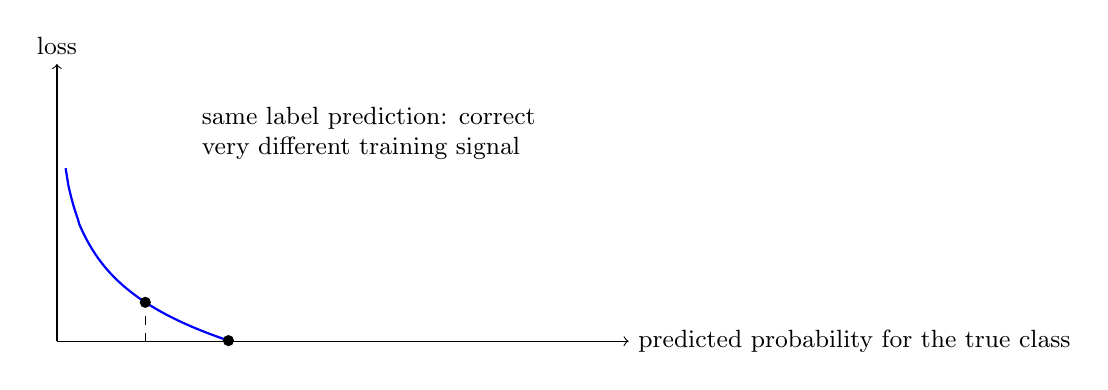
\begin{tikzpicture}[x=2.2cm,y=2.2cm,font=\small]
\draw[->] (0,0) -- (3.3,0) node[right] {predicted probability for the true class};
\draw[->] (0,0) -- (0,1.6) node[above] {loss};
\draw[thick,blue,domain=0.05:0.99,samples=120] plot (\x,{-(ln(\x))/3});
\draw[dashed] (0.51,0) -- (0.51,0.224);
\draw[dashed] (0.99,0) -- (0.99,0.003);
\filldraw (0.51,0.224) circle (1.8pt);
\filldraw (0.99,0.003) circle (1.8pt);
\node[align=left] at (1.8,1.2) {same label prediction: correct\\very different training signal};
\end{tikzpicture}%
}
\caption{Training loss distinguishes weakly correct predictions from confidently correct ones. That is why cross-entropy is useful even when accuracy is the metric reported to an audience.}
\label{fig:same-label-different-loss}
\end{figure}

\subsection{Multiclass Outputs}

Later chapters will repeatedly use multiclass classification, so it is worth seeing the standard pattern now. A multiclass output layer usually produces one raw score per class, called a \emph{logit}, before those scores are normalized into probabilities. In this book, \emph{logit} refers to the raw output of a linear layer before any activation is applied. We sometimes use \emph{score} informally when the distinction does not matter. Softmax converts those logits into probabilities:
\[
\mathrm{softmax}(s)_k = \frac{e^{s_k}}{\sum_j e^{s_j}}.
\]
If the true class is $k^\star$, multiclass cross-entropy penalizes the model according to
\[
\mathcal{L} = -\log \mathrm{softmax}(s)_{k^\star}.
\]

\begin{mathlens}
Softmax is invariant to adding the same constant to every logit. For any scalar \(c\),
\begin{align*}
\mathrm{softmax}(s+c\mathbf{1})_k
&=\frac{e^{s_k+c}}{\sum_j e^{s_j+c}}
=\frac{e^c e^{s_k}}{e^c\sum_j e^{s_j}} \\
&=\mathrm{softmax}(s)_k.
\end{align*}
So only differences between logits matter, not their absolute level. This is why logits are best read as relative evidence before normalization.
\end{mathlens}

\begin{table}[t]
\centering
\small
\begin{tabular}{>{\raggedright}p{1.8cm}>{\centering}p{1.6cm}>{\centering}p{2.5cm}>{\raggedright\arraybackslash}p{3.2cm}}
\toprule
Class & Logit & Softmax prob. & If this is true class \\
\midrule
Class 1 & $1.4$ & $0.654$ & loss contribution $-\log(0.654)\approx 0.425$ \\
Class 2 & $0.5$ & $0.266$ & larger loss if true \\
Class 3 & $-0.7$ & $0.080$ & much larger loss if true \\
\bottomrule
\end{tabular}
\caption{For multiclass problems, logits are not yet probabilities. Softmax turns them into a normalized distribution, and cross-entropy trains the model to place mass on the correct class.}
\label{tab:softmax-example}
\end{table}

\section{Optimization as Repeated Correction}

With the teaching signal now defined, the remaining issue is procedural: how the model uses that signal to improve itself over repeated updates. Training becomes an optimization problem: find parameter values that reduce that loss. Gradient-based optimization works by asking how the loss would change if each parameter were nudged slightly.

\begin{prereqbridge}
A derivative measures local slope. If changing a parameter a little causes the loss to rise sharply, the derivative is large. If changing it causes the loss to fall, the derivative has the opposite sign. A gradient is the collection of these slopes across many parameters.
\end{prereqbridge}

Suppose a one-parameter model predicts $\hat{y}=wx$ and uses squared error:
\[
L = (wx - y)^2.
\]
Take one example with $x=2$, $y=6$, and current parameter $w=1$. Then
\[
\hat{y}=2, \qquad L=(2-6)^2=16.
\]
The derivative with respect to $w$ is
\[
\frac{dL}{dw}=2(wx-y)x.
\]
Substituting the current values gives
\[
\frac{dL}{dw}=2(2-6)(2)=-16.
\]
The negative sign says that increasing $w$ will reduce the loss. If the learning rate is $\eta=0.1$, one gradient descent step gives
\[
w_{\text{new}} = w - \eta \frac{dL}{dw}
= 1 - 0.1(-16)
= 2.6.
\]

\begin{figure}[t]
\centering
\resizebox{\linewidth}{!}{%
\definecolor{c6contOuter}{RGB}{220,233,251}
\definecolor{c6contMid}{RGB}{170,200,240}
\definecolor{c6contInner}{RGB}{120,165,220}
\definecolor{c6contCore}{RGB}{56,103,170}
\definecolor{c6stepBlue}{RGB}{30,80,160}
\begin{tikzpicture}[x=1.8cm,y=1.8cm,font=\small]
%% Filled contour rings (outer to inner)
\fill[c6contOuter]  (0,0) ellipse ({1.5*2.6} and {2.6});
\fill[c6contMid]    (0,0) ellipse ({1.5*2.0} and {2.0});
\fill[c6contInner]  (0,0) ellipse ({1.5*1.4} and {1.4});
\fill[c6contCore!30](0,0) ellipse ({1.5*0.8} and {0.8});
\fill[white]         (0,0) ellipse ({1.5*0.35} and {0.35});
%% Contour outlines
\foreach \r in {0.8,1.4,2.0,2.6}
  \draw[white, line width=0.6pt] (0,0) ellipse ({1.5*\r} and {\r});
%% Gradient descent path
\filldraw[fill=white, draw=c6stepBlue, thick] (-2.4,1.6) circle (3pt);
\draw[-Latex, c6stepBlue, thick, line width=1.2pt] (-2.4,1.6) -- (-1.5,1.0);
\draw[-Latex, c6stepBlue, thick, line width=1.2pt] (-1.5,1.0) -- (-0.8,0.5);
\draw[-Latex, c6stepBlue, thick, line width=1.2pt] (-0.8,0.5) -- (-0.25,0.18);
\filldraw[c6stepBlue] (-1.5,1.0) circle (2pt);
\filldraw[c6stepBlue] (-0.8,0.5) circle (2pt);
%% Minimum marker
\filldraw[fill=white, draw=black, thick] (0,0) circle (2.5pt);
\node[font=\small\bfseries, black!70] at (0.0,-0.55) {minimum};
%% Labels
\node[font=\footnotesize, c6stepBlue, anchor=south] at (-2.4,1.85) {start};
\node[font=\small, black!60, anchor=south west] at (-2.8,2.8) {follow the local slope};
%% Loss level labels - right side, stacked vertically
\node[font=\footnotesize, black!50, anchor=west] at (4.2, 1.0) {\textit{higher loss}};
\draw[->, thin, black!40] (4.1, 1.0) -- (3.4, 1.0);
\node[font=\footnotesize, black!50, anchor=west] at (4.2,-1.0) {\textit{lower loss}};
\draw[->, thin, black!40] (4.1,-1.0) -- (1.6,-0.55);
\end{tikzpicture}%
}
\caption{Gradient descent is repeated local correction, not global magic. Each update uses nearby slope information to move toward lower loss.}
\label{fig:gradient-descent-surface}
\end{figure}

The operational pipeline of training is then:
\begin{itemize}[leftmargin=*]
\item compute a forward pass,
\item compute a loss,
\item push error information backward,
\item update parameters,
\item check validation behavior.
\end{itemize}

Every later training detail in the chapter---learning rate, AdamW, mini-batches, batch normalization, and regularization---modifies this loop rather than replacing it.

\begin{practicalnote}
\textbf{Core loop first, tools second.} The minimum mental model is forward pass, loss, gradient signal, parameter update, and validation check. Optimizers, normalization layers, residual connections, dropout, augmentation, and schedules are tools for making that loop behave better. Students should be able to explain the loop before trying to remember the tool list.
\end{practicalnote}

\begin{codeexample}[caption={A generic neural training loop}]
initialize parameters
for epoch in range(num_epochs):
    for batch in training_data:
        predictions = model(batch.inputs)
        loss = objective(predictions, batch.targets)
        compute gradients of loss with respect to parameters
        update parameters using optimizer
    evaluate on validation data
\end{codeexample}

\begin{figure}[t]
\centering
\resizebox{\linewidth}{!}{%
\begin{tikzpicture}[
  x=1cm,
  y=1cm,
  font=\small,
  box/.style={draw, rounded corners, align=center, minimum width=2.35cm, minimum height=0.85cm},
  note/.style={font=\footnotesize, text=black!70}
]
\node[box] (data) at (0,0) {load batch};
\node[box] (forward) at (3.1,0) {forward pass};
\node[box] (loss) at (6.2,0) {compute loss};
\node[box] (backward) at (9.3,0) {backward pass};
\node[box] (update) at (12.4,0) {update weights};
\node[box] (validate) at (6.2,-2.25) {validation check};

\draw[-Latex, thick] (data) -- (forward);
\draw[-Latex, thick] (forward) -- (loss);
\draw[-Latex, thick] (loss) -- (backward);
\draw[-Latex, thick] (backward) -- (update);

\draw[-Latex, thick] (update.south) |- node[pos=0.22, right, note] {after last batch} (validate.east);
\draw[-Latex, thick] (validate.west) -| node[pos=0.22, below, note] {start next epoch} (data.south);

\draw[rounded corners=6pt, dashed, black!35] (-1.35,0.95) rectangle (13.75,-0.95);
\node[note] at (6.2,1.35) {repeat across training batches inside one epoch};
\end{tikzpicture}%
}
\caption{The training loop is short, but each stage has a distinct role. Batch updates repeat inside an epoch, and validation is checked after the training batches for that epoch. Students should be able to explain what changes during the forward pass, backward pass, and update step.}
\label{fig:training-loop-flow}
\end{figure}

\subsection{Learning Rate}

The learning rate controls step size. If it is too small, training can become painfully slow. If it is too large, optimization can overshoot good regions and become unstable. This is one reason neural training is partly a modeling problem and partly an optimization problem. The architecture may be sound while the training procedure is poor.

\begin{practicalnote}
In practice, the learning rate is rarely held constant. Common schedules include \emph{step decay} (halving the rate every $k$ epochs), \emph{cosine annealing} (smoothly decreasing to near zero), and \emph{warmup} (starting small and ramping up before decaying). The right schedule depends on the problem; the key insight is that the best rate for early training is often too large for fine-tuning near a minimum.
\end{practicalnote}

\begin{figure}[t]
\centering
\definecolor{c6lrSlow}{RGB}{56,103,170}
\definecolor{c6lrGood}{RGB}{26,112,64}
\definecolor{c6lrFast}{RGB}{180,40,40}
\definecolor{c6lrSlowBg}{RGB}{220,233,251}
\definecolor{c6lrGoodBg}{RGB}{210,238,220}
\definecolor{c6lrFastBg}{RGB}{254,216,216}
\resizebox{\linewidth}{!}{%
\begin{tikzpicture}[x=1.4cm,y=3.0cm,font=\small,
  panel/.style={rounded corners=4pt}]
%% ── Panel A: too small ──────────────────────────────────────
\begin{scope}
  \fill[c6lrSlowBg, panel] (-3.4,-0.5) rectangle (3.4,4.4);
  \node[c6lrSlow, font=\small\bfseries] at (0,4.0) {too small};
  \draw[->,black!60] (-3.0,0) -- (3.0,0);
  \draw[->,black!60] (0,0) -- (0,3.6) node[above right, font=\footnotesize, black!50] {loss};
  \draw[black!40, thick, domain=-2.6:2.6, samples=60] plot (\x,{0.4*\x*\x + 0.3});
  %% Tiny steps barely moving
  \filldraw[fill=white, draw=c6lrSlow, thick] (-2.0,1.9) circle (2.5pt);
  \filldraw[c6lrSlow] (-1.6,1.32) circle (2pt);
  \filldraw[c6lrSlow] (-1.3,0.98) circle (2pt);
  \filldraw[c6lrSlow] (-1.05,0.74) circle (2pt);
  \draw[-Latex, c6lrSlow, thick, line width=1.1pt] (-2.0,1.9) -- (-1.6,1.32);
  \draw[-Latex, c6lrSlow, thick, line width=1.1pt] (-1.6,1.32) -- (-1.3,0.98);
  \draw[-Latex, c6lrSlow, thick, line width=1.1pt] (-1.3,0.98) -- (-1.05,0.74);
  \node[font=\footnotesize, c6lrSlow] at (1.5,2.4) {slow progress};
\end{scope}
%% ── Panel B: good ───────────────────────────────────────────
\begin{scope}[xshift=7.5cm]
  \fill[c6lrGoodBg, panel] (-3.4,-0.5) rectangle (3.4,4.4);
  \node[c6lrGood, font=\small\bfseries] at (0,4.0) {good};
  \draw[->,black!60] (-3.0,0) -- (3.0,0);
  \draw[->,black!60] (0,0) -- (0,3.6) node[above right, font=\footnotesize, black!50] {loss};
  \draw[black!40, thick, domain=-2.6:2.6, samples=60] plot (\x,{0.4*\x*\x + 0.3});
  %% Smooth convergence
  \filldraw[fill=white, draw=c6lrGood, thick] (-2.0,1.9) circle (2.5pt);
  \filldraw[c6lrGood] (-0.8,0.56) circle (2pt);
  \filldraw[c6lrGood] (-0.15,0.31) circle (2pt);
  \draw[-Latex, c6lrGood, thick, line width=1.1pt] (-2.0,1.9) -- (-0.8,0.56);
  \draw[-Latex, c6lrGood, thick, line width=1.1pt] (-0.8,0.56) -- (-0.15,0.31);
  \node[font=\footnotesize, c6lrGood] at (1.5,2.4) {steady descent};
\end{scope}
%% ── Panel C: too large ──────────────────────────────────────
\begin{scope}[xshift=15cm]
  \fill[c6lrFastBg, panel] (-3.4,-0.5) rectangle (3.4,4.4);
  \node[c6lrFast, font=\small\bfseries] at (0,4.0) {too large};
  \draw[->,black!60] (-3.0,0) -- (3.0,0);
  \draw[->,black!60] (0,0) -- (0,3.6) node[above right, font=\footnotesize, black!50] {loss};
  \draw[black!40, thick, domain=-2.6:2.6, samples=60] plot (\x,{0.4*\x*\x + 0.3});
  %% Overshooting, bouncing
  \filldraw[fill=white, draw=c6lrFast, thick] (-2.0,1.9) circle (2.5pt);
  \filldraw[c6lrFast] (1.6,1.32) circle (2pt);
  \filldraw[c6lrFast] (-1.4,1.08) circle (2pt);
  \draw[-Latex, c6lrFast, thick, line width=1.1pt] (-2.0,1.9) -- (1.6,1.32);
  \draw[-Latex, c6lrFast, thick, line width=1.1pt] (1.6,1.32) -- (-1.4,1.08);
  \node[font=\footnotesize, c6lrFast] at (1.5,2.4) {overshoots};
\end{scope}
\end{tikzpicture}%
}
\caption{Step size is part of the training design. Too small wastes computation, while too large can bounce across good regions instead of settling into them.}
\label{fig:learning-rate-cases}
\end{figure}

\subsection{Adaptive Optimization: Momentum, Adam, and AdamW}

The learning rate tells us how large a step to take, but it does not say how to shape the step when the loss surface is uneven. Adaptive optimizers try to make optimization less brittle by using recent gradient information to smooth motion or scale updates per parameter.

\textbf{Momentum} accumulates a running direction of travel. If successive gradients point roughly the same way, momentum keeps the update moving that way instead of restarting from scratch at every batch. If gradients alternate direction, momentum damps the zig-zag. The idea is simple: do not treat the latest gradient as the entire story.

\textbf{Adam} adds a second idea: keep running statistics of both the gradient and its squared magnitude. The first statistic tracks direction, and the second tracks scale. Parameters with consistently large gradients get smaller effective steps; parameters with consistently small or noisy gradients get more usable steps. In practice, this often makes early training easier and less sensitive to a single global step size.

\textbf{AdamW} is Adam with decoupled weight decay: it keeps the adaptive step logic but separates weight decay from the gradient update itself. That separation matters because weight decay is a regularization choice, not a disguised learning-rate trick. Students should think of AdamW as saying: ``adapt the step, but still regularize the weights in the intended way.''

\begin{example}[A One-Coordinate Optimizer Intuition]
Suppose one weight sees successive gradients \(8,7,9\), while another sees \(0.2,0.1,0.3\). Plain gradient descent uses the same global learning rate on both coordinates. Momentum treats the first sequence as persistent downhill evidence and keeps velocity in that direction instead of restarting every step. Adam goes further and rescales the coordinates differently: the large-gradient weight receives a more conservative effective step, while the small-gradient weight is not drowned out entirely by the same global rate. The point is not that Adam knows the right answer. The point is that different coordinates can require different step behavior.
\end{example}

\begin{codeexample}[caption={A compact adaptive-update skeleton}]
initialize parameters
initialize first_moment and second_moment to zero
initialize timestep = 0
for each minibatch gradient grad:
    timestep = timestep + 1
    reference_parameters = parameters
    first_moment = beta1 * first_moment + (1 - beta1) * grad
    second_moment = beta2 * second_moment + (1 - beta2) * (grad * grad)
    debiased_first = first_moment / (1 - beta1^timestep)
    debiased_second = second_moment / (1 - beta2^timestep)
    parameters = parameters - learning_rate * debiased_first / (sqrt(debiased_second) + epsilon)
    if using AdamW:
        parameters = parameters - learning_rate * weight_decay * reference_parameters
\end{codeexample}

\begin{practicalnote}
Momentum and Adam-like methods help most when optimization is noisy, poorly scaled, or sensitive to a single global step size. They do not fix label noise, leakage, a broken loss-output match, or a model that is simply too weak to represent the task.
\end{practicalnote}

\begin{example}[When Adam Helps and When It Does Not]
Suppose a model trains erratically because different parameters receive gradients on very different scales. Adam often stabilizes that situation quickly. But if the labels are wrong or the output layer does not match the task, Adam can still produce a confident failure faster than SGD. A better optimizer is not a substitute for a correct problem formulation.
\end{example}

\subsection{Optimization Failure Versus Generalization Failure}

When a neural network performs poorly, the cause is usually one of two fundamentally different problems. Conflating them leads to wasted effort because the remedies are different.

\textbf{Optimization failure} means the model cannot fit the training signal at all. Training loss stays high, barely decreases, or fluctuates without settling. The model is not learning the mapping the data contains. Common causes include a learning rate that is too large or too small, a weight initialization that puts the network in a poor region, a mismatch between the output layer and the loss function, or label corruption that prevents any consistent rule from forming.

\textbf{Generalization failure} means the model fits the training data well but fails on new examples. Training loss is low; validation loss is high or diverges from training loss as training continues. The model is memorizing rather than learning a pattern that transfers. Common causes include a model with too much capacity relative to the dataset size, insufficient regularization, insufficient data augmentation, or distribution shift between training and deployment.

\begin{table}[t]
\centering
\small
\setlength{\tabcolsep}{4pt}
\begin{tabular}{p{2.77cm}p{2.06cm}p{2.06cm}p{2.77cm}}
\toprule
Failure type & Training loss & Validation loss & Where to look \\
\midrule
Optimization failure & High & High & Learning rate, initialization, output layer, label noise \\
Generalization failure & Low & High & Capacity, regularization, data size, augmentation \\
Both & High & High & Fix optimization first, then assess generalization \\
\bottomrule
\end{tabular}
\caption{Diagnosing the failure type before applying remedies saves considerable effort. Regularization does not help when the model cannot fit its training data.}
\label{tab:opt-vs-gen-failure}
\end{table}

This distinction is foundational for debugging. Students who do not draw it clearly will add dropout when they should be fixing the output layer, or increase model capacity when they should be adding regularization. Both changes would be reasonable in other contexts, but neither is helpful when applied to the wrong failure type. The first debugging reflex in this chapter should therefore be diagnostic, not architectural.

The cleanest diagnostic procedure is to first establish whether the model can overfit a very small dataset. Take a batch of ten to twenty training examples and train the model until training loss is very low. If the model cannot overfit even ten examples, the problem is optimization. If it can overfit ten examples but not generalize on the full dataset, the problem is generalization. The separation is not always perfect, but the small-batch overfit test is the fastest way to decide which problem to solve first.

\subsection{Mini-Batches, Initialization, and Stability}

In principle, gradients could be computed using the entire training set before every update. In practice, that is often too expensive. Instead, we use mini-batches: small subsets of examples that produce noisy but useful gradient estimates. This gives rise to stochastic gradient descent and its many variants.

\begin{figure}[t]
\centering
\resizebox{\linewidth}{!}{%
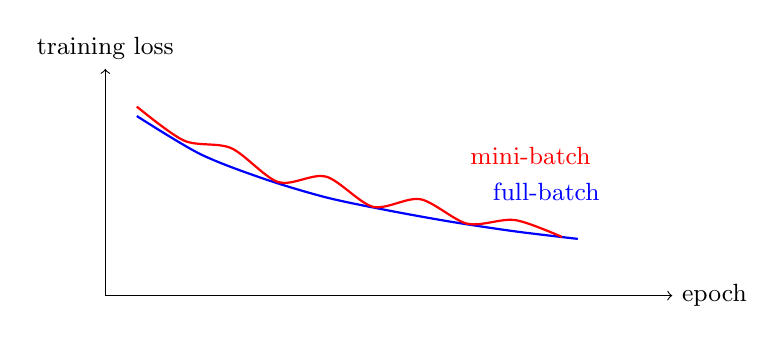
\begin{tikzpicture}[x=1.0cm,y=2.4cm,font=\small]
\draw[->] (0,0) -- (7.2,0) node[right] {epoch};
\draw[->] (0,0) -- (0,1.2) node[above] {training loss};
\draw[thick,blue] plot[smooth] coordinates {(0.4,0.95) (1.2,0.75) (2.0,0.62) (2.8,0.52) (3.6,0.45) (4.4,0.39) (5.2,0.34) (6.0,0.30)};
\draw[thick,red] plot[smooth] coordinates {(0.4,1.00) (1.0,0.82) (1.6,0.78) (2.2,0.60) (2.8,0.63) (3.4,0.47) (4.0,0.51) (4.6,0.38) (5.2,0.40) (5.8,0.31)};
\node[blue] at (5.6,0.55) {full-batch};
\node[red] at (5.4,0.74) {mini-batch};
\end{tikzpicture}%
}
\caption{Mini-batch updates usually make optimization noisier than full-batch updates. That noise is often acceptable and sometimes beneficial, but it changes how training curves should be read.}
\label{fig:full-batch-vs-minibatch}
\end{figure}

Training also does not begin from nowhere. Parameters must be initialized, inputs must be scaled sensibly, and layers must receive signals of a manageable size. Bad initialization can produce activations that are too small, too large, or too similar, making optimization slow or unstable from the first step.

\begin{mathlens}
If two hidden units start with exactly the same weights and bias, then they compute the same pre-activation on every example, produce the same activation, and receive the same gradient update. Gradient descent preserves that equality, so the two units never specialize; the network learns one feature twice. Random initialization breaks that symmetry by giving each unit a slightly different starting point, which lets different hidden units move toward different useful features.
\end{mathlens}

\begin{example}[Three Bad Starts]
If every hidden unit starts at zero, the layer stays symmetric and learns duplicate features. If the initial weights are extremely small, signals shrink as they pass through many layers and learning becomes sluggish. If the initial weights are extremely large, activations or gradients can explode or saturate. Good initialization is therefore about scale and diversity at the same time. In practice, initialization schemes such as He initialization (for ReLU networks) and Xavier initialization (for sigmoid/tanh networks) have been developed to keep activations and gradients in a reasonable range through early training. Most frameworks apply sensible defaults, but awareness of the issue helps when debugging slow or unstable convergence.
\end{example}

\begin{warningbox}
When students say ``the network did not work,'' the failure may be in the learning rate, initialization, batch setup, or data preprocessing rather than in the idea of the model itself.
\end{warningbox}

\begin{practicalnote}
If a neural model fails early, check simple stability questions before redesigning the architecture: Were the inputs normalized? Is the learning rate reasonable? Are the initial weights making activations explode or vanish? Is the batch size so small that the gradients are mostly noise?
\end{practicalnote}

\subsection{Batch Normalization as Signal Stabilization}

Batch normalization is another way to make optimization less brittle. It is a training-time rescaling step that normalizes intermediate activations using statistics computed from the current mini-batch, then restores flexibility with learned scale and shift parameters. The intuition is that if the hidden signals stay in a manageable range, the next layers see a more stable training problem.

That description is enough for this book. Students do not need to memorize the exact implementation before they understand the purpose: batch normalization reduces internal scale drift, which can make optimization smoother and allow somewhat larger learning rates. It is a training aid, not a cure-all.

\begin{mathlens}
For mini-batch activations \(a_1,\ldots,a_m\), batch normalization computes
\[
\hat a_i = \frac{a_i-\mu_B}{\sqrt{\sigma_B^2+\varepsilon}},
\qquad
b_i = \gamma \hat a_i + \beta,
\]
where \(\mu_B\) and \(\sigma_B^2\) are the batch mean and variance, and \(\gamma,\beta\) are learned scale and shift parameters. The normalization stabilizes the signal; the learned affine step keeps the layer expressive.
\end{mathlens}

\begin{practicalnote}
During training, batch normalization uses statistics (mean and variance) computed from the current mini-batch. At inference time, the model instead uses running averages accumulated during training. This asymmetry means that a model can behave differently in training and inference modes---a source of subtle bugs when deploying neural networks. Always verify that your framework is set to evaluation mode before serving predictions.
\end{practicalnote}

\begin{figure}[t]
\centering
\resizebox{\linewidth}{!}{%
\begin{tikzpicture}[x=1cm,y=1cm,font=\small,
  box/.style={draw, rounded corners, align=center, minimum width=2.7cm, minimum height=0.9cm, fill=black!4}]
\node[box] (raw) at (0,0) {hidden activations};
\node[box] (norm) at (4.0,0) {normalize\\by batch statistics};
\node[box] (scale) at (8.0,0) {learned scale\\and shift};
\node[box] (next) at (12.0,0) {more stable\\next layer};
\draw[-Latex, thick] (raw) -- (norm);
\draw[-Latex, thick] (norm) -- (scale);
\draw[-Latex, thick] (scale) -- (next);
\end{tikzpicture}%
}
\caption{Batch normalization aims to stabilize the signal passing through the network so later layers do not have to adapt to wildly changing activation scales.}
\label{fig:batch-norm-stability}
\end{figure}

\begin{example}[What Batch Normalization Fixes, and What It Does Not]
If hidden activations are drifting in scale from batch to batch, batch normalization can make training smoother and less sensitive to the exact learning rate. For a mini-batch with activations \(2,4,6\), the layer first recenters them around zero before the learned rescaling step. The next layer therefore reacts to relative variation rather than raw drift in magnitude. But batch normalization still does not fix a wrong objective, a poor label set, or a model that lacks the capacity to learn the task in the first place.
\end{example}

\begin{practicalnote}
Batch normalization stabilizes the signal within a layer. A complementary technique called a \emph{residual connection} (or skip connection) helps the signal flow between layers. When the shapes match, instead of computing $h = f(x)$, the layer computes $h = f(x) + x$, adding the input directly to the output. When the shapes do not match, architectures typically insert a projection on the skip path before adding. If the transformation $f$ is unhelpful, the gradient can flow through the identity or projected branch, so deep networks become much easier to train. Residual connections are a key design principle behind ResNets in vision and many transformer blocks in language.
\end{practicalnote}

\subsection{Debugging a Broken Training Run}

Students often respond to a bad neural result by changing the architecture first. That is usually too early. The more disciplined first question is: what kind of failure are we seeing?

\begin{table}[t]
\centering
\small
\setlength{\tabcolsep}{4pt}
\begin{tabular}{@{}>{\raggedright\arraybackslash}p{3.41cm}>{\raggedright\arraybackslash}p{3.33cm}>{\raggedright\arraybackslash}p{3.49cm}@{}}
\toprule
Observed pattern & First interpretation to test & Better first response than ``change the architecture'' \\
\midrule
Training loss hardly moves & optimization setup may be broken & check loss-output alignment, learning rate, normalization, and whether the model can overfit one tiny batch \\
Training loss falls but validation is poor & optimization is working but generalization is weak & inspect data quality, regularization, augmentation, label noise, and evaluation split logic \\
Loss becomes NaN or oscillates wildly & updates are unstable & lower the learning rate, inspect initialization, check activation scale, and verify preprocessing \\
Training and validation both look strangely strong immediately & leakage or target mismatch may exist & audit splits, labels, duplicated examples, and feature construction before celebrating \\
\bottomrule
\end{tabular}
\caption{Neural debugging improves when students distinguish optimization failure from generalization failure instead of treating every weak result as an architecture problem.}
\label{tab:neural-debugging-patterns}
\end{table}

This distinction is foundational. If the network cannot even reduce the training objective, then there is no point debating whether it overfits. If it fits training well but collapses on validation, then the training loop is not the first suspect. Different failures demand different questions.

\begin{codeexample}[caption={A minimal debugging sequence before redesigning the network}]
pick one tiny batch of examples
verify that targets, output layer, and loss function match
try to overfit that tiny batch nearly perfectly
if this fails:
    inspect learning rate, normalization, initialization, and gradient scale
if this succeeds but validation is weak:
    inspect data quality, slice coverage, regularization, and leakage
change one training choice at a time and record the effect
\end{codeexample}

The tiny-batch test is especially valuable because it removes excuses. A reasonably implemented network with aligned outputs and targets should usually be able to memorize a very small batch. If it cannot, the problem is often in the training setup rather than in the grand modeling idea.

\begin{practicalnote}
A simple practical remedy for exploding gradients is \emph{gradient clipping}: if the norm of the gradient vector exceeds a threshold, rescale it to that threshold before applying the update. This does not fix the underlying cause, but it prevents catastrophically large steps.
\end{practicalnote}

\begin{decisionbox}
Before increasing model depth or width, ask whether the run failed because the model could not fit the training signal at all, or because it fit the training signal and failed to generalize. Those are different problems and should trigger different interventions.
\end{decisionbox}

\begin{thinkingtool}
\textbf{Tempting mistake $\rightarrow$ corrected reasoning.} Tempting mistake: ``Validation is bad, so the architecture must be wrong.'' Corrected reasoning: ``First separate optimization failure from generalization failure. If the network cannot overfit a tiny batch, debug the training setup. If it can, inspect data quality, split logic, regularization, and evaluation before redesigning the model family.''
\end{thinkingtool}

Once the training loop behaves sensibly, the remaining conceptual question is how the error signal reaches the earlier layers that created the internal representation in the first place.

\section{Backpropagation as Credit Assignment}

\begin{definition}[Backpropagation]
Backpropagation is the efficient procedure for computing how the loss changes with respect to every parameter in a layered network by repeatedly applying the chain rule from the output layer backward.
\end{definition}

Conceptually, backpropagation solves one clear problem: when the network makes an error, which earlier computations deserve credit or blame, and by how much?

\begin{practicalnote}
Backpropagation is efficient because it requires only one forward pass and one backward pass to compute gradients for \emph{every} parameter simultaneously. The naive alternative---perturbing each parameter individually and measuring the change in loss---would require one forward pass per parameter, making it impractical for networks with millions of weights.
\end{practicalnote}

\begin{figure}[t]
\centering
\definecolor{c6fwdBlue}{RGB}{56,103,170}
\definecolor{c6bwdRed}{RGB}{180,40,40}
\resizebox{\linewidth}{!}{%
\begin{tikzpicture}[x=1cm, y=1cm, font=\small,
  circ/.style={draw=black!70, circle, minimum size=0.85cm, thick, fill=white}
]
%% Chain nodes on a horizontal track at y=2.0
%% Inputs stacked to the left at x=0; z merges them at x=2.8
\node[circ] (x1) at (0.0, 3.0) {$x_1$};
\node[circ] (x2) at (0.0, 1.0) {$x_2$};
\node[circ] (z)  at (3.2, 2.0) {$z$};
\node[circ] (h)  at (6.0, 2.0) {$h$};
\node[circ] (s)  at (8.8, 2.0) {$s$};
\node[circ] (l)  at (11.6,2.0) {$L$};

%% ---- Forward pass: blue arrows running ABOVE the node centres ----
\draw[-Latex, thick, c6fwdBlue] (x1) -- (z);
\draw[-Latex, thick, c6fwdBlue] (x2) -- (z);
%% Arrows along chain with labels ABOVE the arrows
\draw[-Latex, thick, c6fwdBlue] (z) --
  node[above, font=\footnotesize, c6fwdBlue] {ReLU} (h);
\draw[-Latex, thick, c6fwdBlue] (h) -- (s);
\draw[-Latex, thick, c6fwdBlue] (s) -- (l);

%% ---- Backward pass: red dashed arrows looping FAR BELOW ----
%% Use large bend so arcs clear the node circles completely
\draw[-Latex, thick, c6bwdRed, dashed]
  (l.south) .. controls (10.2,0.2) and (9.4,0.2) .. (s.south);
\node[c6bwdRed, font=\footnotesize] at (10.2, -0.1) {$\tfrac{dL}{ds}$};

\draw[-Latex, thick, c6bwdRed, dashed]
  (s.south) .. controls (7.4,0.0) and (6.6,0.0) .. (h.south);
\node[c6bwdRed, font=\footnotesize] at (7.4, -0.3) {$\tfrac{dL}{dh}$};

\draw[-Latex, thick, c6bwdRed, dashed]
  (h.south) .. controls (4.6,0.0) and (3.8,0.0) .. (z.south);
\node[c6bwdRed, font=\footnotesize] at (4.6, -0.3) {$\tfrac{dL}{dz}$};

%% From z back to inputs - route below to avoid "input gradients" label
\draw[-Latex, thick, c6bwdRed, dashed]
  (z.west) .. controls (2.0,1.2) and (0.8,1.2) .. (x1.south);
\draw[-Latex, thick, c6bwdRed, dashed]
  (z.west) .. controls (2.0,0.6) and (0.8,0.6) .. (x2.south);
%% "input gradients" label placed below x2, clear of all arrows
\node[c6bwdRed, font=\footnotesize, align=center] at (1.3, -0.3)
  {input gradients};

%% ---- Section labels ----
\node[c6fwdBlue, font=\small\bfseries] at (5.8, 4.2) {forward computation};
\node[c6bwdRed,  font=\small\bfseries] at (7.5,-1.2) {backward credit assignment};
\end{tikzpicture}%
}
\caption{Backpropagation is easiest to understand as a computational graph. The forward pass creates values; the backward pass distributes the loss signal through those same dependencies in reverse.}
\label{fig:computational-graph-backprop}
\end{figure}

\subsection{A Small Worked Gradient Example}

The next calculation intentionally switches to a one-hidden-unit squared-error network so that every derivative fits on the page. It is a side example for the mechanics of backpropagation, not a replacement for the running spam classifier. The same reverse-credit idea applies to the sigmoid cross-entropy network above; only the local derivatives change.

Consider a network with one ReLU hidden unit:
\[
z = w_1x_1 + w_2x_2 + b_h,
\qquad
h = \mathrm{ReLU}(z),
\]
\[
s = vh + b_o,
\qquad
L = \frac{1}{2}(s-y)^2.
\]
Take one example with input $(x_1,x_2)=(2,1)$ and target $y=1$. Let the current parameter values be
\begin{align*}
w_1 &= 0.5, & w_2 &= 1.0, & b_h &= -1.0, \\
v   &= 1.2, & b_o &= -0.3.
\end{align*}

First perform the forward pass:
\[
z = 0.5(2) + 1.0(1) - 1.0 = 1,
\qquad
h = \mathrm{ReLU}(1)=1,
\]
\[
s = 1.2(1) - 0.3 = 0.9,
\qquad
L = \frac{1}{2}(0.9-1)^2 = 0.005.
\]

Now move backward through the computation. Start with the loss derivative with respect to the score:
\[
\frac{dL}{ds} = s-y = 0.9-1 = -0.1.
\]
This says increasing the score slightly would reduce the loss.

The output weight $v$ multiplies $h$, so
\[
\frac{dL}{dv} = \frac{dL}{ds}\cdot h = (-0.1)(1) = -0.1.
\]
The hidden activation affects the loss through the output layer, so
\[
\frac{dL}{dh} = \frac{dL}{ds}\cdot v = (-0.1)(1.2) = -0.12.
\]
Because $z=1>0$, the derivative of ReLU at this point is $1$, so
\[
\frac{dL}{dz} = \frac{dL}{dh}\cdot 1 = -0.12.
\]
Now the hidden-layer parameters follow directly:
\[
\frac{dL}{dw_1} = \frac{dL}{dz}\cdot x_1 = (-0.12)(2) = -0.24,
\]
\[
\frac{dL}{dw_2} = \frac{dL}{dz}\cdot x_2 = (-0.12)(1) = -0.12,
\]
\[
\frac{dL}{db_h} = \frac{dL}{dz} = -0.12.
\]

The output bias behaves similarly:
\[
\frac{dL}{db_o} = \frac{dL}{ds} = -0.1.
\]

This is backpropagation in miniature. The error signal begins at the loss, flows backward through the output computation, then through the activation, and finally into the earlier weights and bias.

To make that chain feel like learning rather than bookkeeping, take one gradient-descent step with learning rate \(\eta = 0.05\):
\[
w_1' = 0.512, \quad w_2' = 1.006,
\]
\[
b_h' = -0.994, \quad v' = 1.205,
\]
\[
b_o' = -0.3 - 0.05(-0.1) = -0.295.
\]
Now rerun the same example with the updated parameters:
\begin{align*}
z' &= 0.512(2) + 1.006(1) - 0.994 = 1.036, \\
h' &= \mathrm{ReLU}(1.036) = 1.036,
\end{align*}
\begin{align*}
s' &= 1.205(1.036) - 0.295 \approx 0.953, \\
L' &= \tfrac{1}{2}(0.953-1)^2 \approx 0.0011.
\end{align*}
The loss fell from \(0.005\) to about \(0.0011\) after one step. That does not prove the network will generalize, but it does show the operational meaning of the gradients we just computed: they point toward a local parameter change that improves this example.

\subsection{What Changes If ReLU Is Off?}

Now imagine the same network but with a hidden pre-activation $z=-0.5$. Then $h=\mathrm{ReLU}(-0.5)=0$, and because $z<0$ the local derivative of ReLU is exactly $0$ at that point. The non-differentiability issue appears at $z=0$, not at negative inputs such as this one. The backward chain therefore gives
\[
\frac{dL}{dz} = \frac{dL}{dh}\cdot 0 = 0.
\]
The gradients into the earlier hidden-layer weights also become zero for that example. This is a useful practical fact: whether a ReLU unit is active changes not just the forward value, but whether gradient signal can flow through that pathway on that example.

\begin{failurebox}
Backpropagation does not guarantee good learning. It only tells us the local direction of improvement. If the data is weak, the model is badly chosen, the learning rate is poor, or the objective is mismatched to the task, the network can still fail badly while all gradients are computed correctly.
\end{failurebox}

\begin{advancednote}
In real implementations, these gradient calculations are handled by automatic differentiation systems. That convenience is useful, but students should still understand the manual logic. Otherwise training becomes a black box: loss goes in, gradients come out, and no one can explain why.
\end{advancednote}

\begin{codeexample}[caption={From scratch: one backpropagation step through the output layer}]
# Continue from the forward pass above.
# Restate the values computed there for clarity.
# h1, h2: hidden unit activations (post-ReLU)
# v1, v2, b_out: output-layer weights and bias
# s: output score (pre-sigmoid);  p: predicted probability
# y: true label (1 = positive class)
y = 1

# --- Binary cross-entropy loss (single example) ---
# L = -(y * log(p) + (1-y) * log(1-p))
import math
loss = -(y * math.log(p) + (1 - y) * math.log(1 - p))
print("binary cross-entropy loss:  ", round(loss, 4))

# --- Gradient at the output layer ---
# For sigmoid + cross-entropy the combined gradient simplifies to (p - y).
dL_ds = p - y          # dL/ds: how the loss changes with the pre-sigmoid score
print("dL/ds (output gradient):    ", round(dL_ds, 4))

# Gradient w.r.t. output weight v1 (chain rule: dL/dv1 = dL/ds * ds/dv1 = dL/ds * h1)
dL_dv1 = dL_ds * h1    # credit assigned to v1
print("dL/dv1:                     ", round(dL_dv1, 4))

# --- Gradient flowing back to hidden unit 1 ---
# dL/dh1 = dL/ds * ds/dh1 = dL/ds * v1
dL_dh1 = dL_ds * v1    # error signal arriving at hidden unit 1
print("dL/dh1:                     ", round(dL_dh1, 4))

# Pass through ReLU: derivative is 1 if h1 > 0, else 0
relu_gate = 1.0 if h1 > 0 else 0.0   # local gradient of ReLU
dL_dz1 = dL_dh1 * relu_gate           # dL/dz1
print("dL/dz1 (through ReLU gate): ", round(dL_dz1, 4))

# Gradient w.r.t. the hidden weight w11 (dL/dw11 = dL/dz1 * dz1/dw11 = dL/dz1 * x1)
dL_dw11 = dL_dz1 * x1
print("dL/dw11:                    ", round(dL_dw11, 4))

# --- One gradient-descent update (learning rate = 0.1) ---
learning_rate = 0.1
new_v1  = v1  - learning_rate * dL_dv1    # output weight update
new_w11 = w11 - learning_rate * dL_dw11   # hidden weight update
print("updated v1:                 ", round(new_v1, 4))
print("updated w11:                ", round(new_w11, 4))
\end{codeexample}

\begin{figure}[t]
\centering
\definecolor{c6fwdBlue}{RGB}{56,103,170}
\definecolor{c6bwdRed}{RGB}{180,40,40}
\definecolor{c6fwdBg}{RGB}{220,233,251}
\definecolor{c6bwdBg}{RGB}{254,230,230}
\resizebox{\linewidth}{!}{%
\begin{tikzpicture}[font=\small,
  fwdarrow/.style={-Latex, thick, c6fwdBlue},
  bwdarrow/.style={-Latex, thick, c6bwdRed},
  box/.style={draw, rounded corners=4pt, align=center, minimum width=2.6cm,
              minimum height=1.1cm, fill=c6fwdBg, draw=c6fwdBlue!60,
              font=\small}]
%% ── Boxes (left to right) ───────────────────────────────────
\node[box] (w)   at (0.0, 0) {input weight\\$w_{11}$};
\node[box] (h)   at (4.0, 0) {hidden unit\\$h_1$};
\node[box] (out) at (8.0, 0) {output unit\\$s$};
\node[box, fill=c6bwdBg, draw=c6bwdRed!50] (L) at (12.0, 0) {loss\\$\mathcal{L}$};
%% ── Forward arrows (top, left to right) ─────────────────────
\draw[fwdarrow] (w.east)   -- node[above, font=\footnotesize, c6fwdBlue] {forward} (h.west);
\draw[fwdarrow] (h.east)   -- node[above, font=\footnotesize, c6fwdBlue] {forward} (out.west);
\draw[fwdarrow] (out.east) -- node[above, font=\footnotesize, c6fwdBlue] {forward} (L.west);
%% ── Backward gradient arrows (staggered depths) ────────────
%% Loss → output (shallowest, y = -1.2)
\draw[c6bwdRed, thick] (L.south) -- ++(0,-0.65) coordinate (bL1);
\draw[bwdarrow] (bL1) -- node[below, font=\footnotesize, c6bwdRed]
    {$\dfrac{\partial\mathcal{L}}{\partial s}=\hat{p}-y$}
    (bL1 -| out.south) coordinate (bO1);
\draw[c6bwdRed, thick, -Latex] (bO1) -- (out.south);
%% Output → hidden (middle, y = -2.0)
\draw[c6bwdRed, thick] ([xshift=-2pt]out.south) -- ++(0,-1.45) coordinate (bO2);
\draw[bwdarrow] (bO2) -- node[below, font=\footnotesize, c6bwdRed]
    {$\dfrac{\partial\mathcal{L}}{\partial h_1}$}
    (bO2 -| h.south) coordinate (bH1);
\draw[c6bwdRed, thick, -Latex] (bH1) -- ([xshift=2pt]h.south);
%% Hidden → input weight (deepest, y = -2.8)
\draw[c6bwdRed, thick] ([xshift=-2pt]h.south) -- ++(0,-2.25) coordinate (bH2);
\draw[bwdarrow] (bH2) -- node[below, font=\footnotesize, c6bwdRed]
    {$\dfrac{\partial\mathcal{L}}{\partial w_{11}}$}
    (bH2 -| w.south) coordinate (bW1);
\draw[c6bwdRed, thick, -Latex] (bW1) -- ([xshift=2pt]w.south);
%% ── Row labels ──────────────────────────────────────────────
\node[font=\footnotesize\bfseries, c6fwdBlue] at (6.0, 1.3) {forward pass};
\node[font=\footnotesize\bfseries, c6bwdRed]  at (6.0,-4.0) {backward pass (gradient flow)};
\end{tikzpicture}%
}
\caption{Backpropagation is credit assignment flowing backward through the network. Each arrow carries the gradient signal that tells one weight how much to adjust.}
\label{fig:backprop-credit-flow}
\end{figure}

\section{Generalization Returns: Regularization as Bias Toward Stable Patterns}

Neural networks are flexible enough to fit very complicated patterns. That flexibility is powerful and dangerous. A large network can capture real structure, but it can also memorize accidents of the training set.

The evaluation-discipline question from Chapter~\ref{ch:evaluation-discipline} returns in sharper form: are we reducing training loss in a way that helps on unseen data, or are we merely fitting noise more effectively?

The best way to understand regularization in this chapter is not as a list of tricks. It is as a bias toward less brittle learned representations. These tools matter after the model can learn; they are not substitutes for fixing a broken optimization setup.

\subsection{Weight Decay, Early Stopping, Dropout, and Augmentation}

Several common tools are used to control overfitting. \textbf{Weight decay} discourages large parameter values by penalizing them during optimization. \textbf{Early stopping} halts training when validation performance stops improving. \textbf{Dropout} randomly suppresses some activations during training so the network does not rely too heavily on any one pathway. \textbf{Data augmentation} expands effective data variety by transforming inputs in label-preserving ways.

These techniques are different in mechanism but similar in purpose. They push the network toward patterns that are stable enough to survive outside the training sample.

Dropout deserves one extra caution. It is useful because it prevents a network from depending too heavily on one hidden pathway, but it does not magically create information that is absent from the data. If the core representation is wrong, dropout only regularizes a bad model.

\begin{example}[What Dropout Actually Changes]
Suppose a hidden layer currently produces activations \((1.2, 0.9, 0.0, 1.1)\). With dropout rate \(0.5\), one training step might keep only the first and fourth activations, while another might keep the second and fourth. The next layer therefore cannot rely on one fragile path always being present. Over many updates, the network is pushed to spread evidence across several features. In standard inverted-dropout implementations, the kept activations are rescaled during training, so at inference time all units are available again and the forward pass is unchanged.
\end{example}

\begin{figure}[t]
\centering
\resizebox{\linewidth}{!}{%
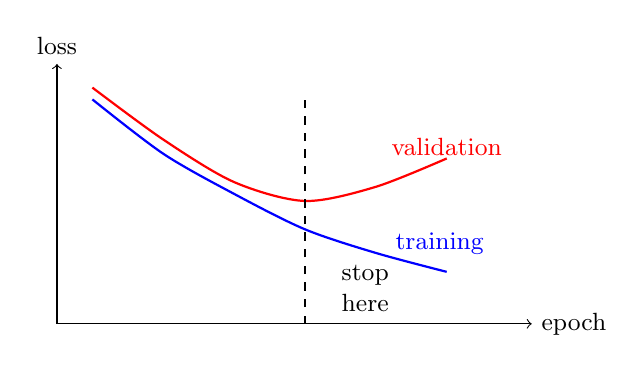
\begin{tikzpicture}[x=0.9cm,y=3.0cm,font=\small]
\draw[->] (0,0) -- (6.7,0) node[right] {epoch};
\draw[->] (0,0) -- (0,1.1) node[above] {loss};
\draw[thick,blue] plot[smooth] coordinates {(0.5,0.95) (1.5,0.72) (2.5,0.55) (3.5,0.40) (4.5,0.30) (5.5,0.22)};
\draw[thick,red] plot[smooth] coordinates {(0.5,1.00) (1.5,0.78) (2.5,0.60) (3.5,0.52) (4.5,0.58) (5.5,0.70)};
\draw[dashed] (3.5,0) -- (3.5,0.95);
\node[blue] at (5.4,0.34) {training};
\node[red] at (5.5,0.75) {validation};
\node[align=center] at (4.35,0.15) {stop\\here};
\end{tikzpicture}%
}
\caption{Early stopping marks the point where additional training mainly improves fit to the seen data rather than generalization to new data.}
\label{fig:early-stopping-curve}
\end{figure}

\begin{figure}[t]
\centering
\definecolor{c6regBg}{RGB}{220,233,251}
\definecolor{c6regLine}{RGB}{56,103,170}
\resizebox{\linewidth}{!}{%
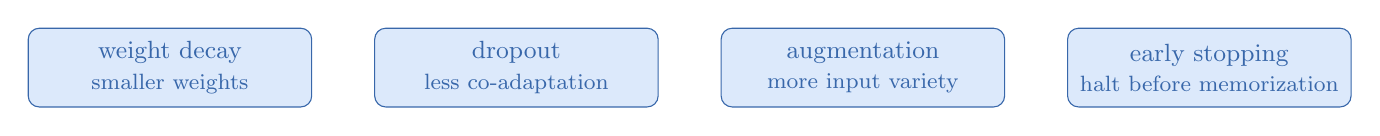
\begin{tikzpicture}[x=1cm, y=1cm, font=\small,
  rbox/.style={draw=c6regLine, fill=c6regBg, rounded corners,
               align=center, minimum width=3.6cm, minimum height=1.0cm,
               text=c6regLine}
]
%% Four boxes spaced 4.4 cm apart (gap = 4.4 - 3.6 = 0.8 cm clear)
\node[rbox] at (0.0, 0) {weight decay\\{\footnotesize smaller weights}};
\node[rbox] at (4.4, 0) {dropout\\{\footnotesize less co-adaptation}};
\node[rbox] at (8.8, 0) {augmentation\\{\footnotesize more input variety}};
\node[rbox] at (13.2,0) {early stopping\\{\footnotesize halt before memorization}};
\end{tikzpicture}%
}
\caption{These regularization tools work differently, but they all try to bias learning toward patterns that remain useful outside the training sample.}
\label{fig:regularization-toolbox}
\end{figure}

\begin{example}[A Familiar Tradeoff]
Suppose an augmented image model scores slightly lower on clean validation images than a non-augmented model, but performs much better on shifted or noisy images. That is not a contradiction. It means the model traded some specialization for robustness. Honest reporting should describe both sides of that tradeoff.
\end{example}

\section{Capacity, Data Regime, and Label Noise}

``Use a bigger model'' is not a universal recommendation. Model capacity interacts with dataset size, label quality, and augmentation quality in ways that make the same capacity increase beneficial in one regime and harmful in another.

\textbf{Large capacity with sufficient clean data.} When the dataset is large and labels are reliable, a higher-capacity model can find finer structure and use its additional parameters productively. Adding layers, widening the network, or removing regularization may all improve performance in this regime because the training signal is abundant and trustworthy.

\textbf{Large capacity with limited clean data.} When the dataset is small or labels are sparse, additional capacity often leads to memorization rather than generalization. The model learns idiosyncratic patterns of the training examples instead of the underlying structure. In this regime, regularization, early stopping, data augmentation, and smaller architectures tend to help more than increasing capacity.

\textbf{High label noise.} When labels contain substantial errors---from careless annotation, ambiguous task definitions, or label leakage---a higher-capacity model is more likely to memorize those errors than a lower-capacity one. The large model has the flexibility to overfit the noise; the small model may not. Label quality should be assessed and improved before architectural decisions are made, because adding layers to fix a label-noise problem usually makes the problem worse.

\begin{figure}[t]
\centering
\resizebox{\linewidth}{!}{%
\begin{tikzpicture}[font=\small, x=3.5cm, y=2.0cm]
\draw[->] (0,0) -- (2.6,0) node[right] {dataset size};
\draw[->] (0,0) -- (0,2.4) node[above] {validation performance};
\draw[thick, blue] plot[smooth] coordinates {(0.1,0.3) (0.5,0.9) (1.0,1.4) (1.8,1.8) (2.4,2.0)};
\draw[thick, red, dashed] plot[smooth] coordinates {(0.1,0.1) (0.5,0.5) (1.0,1.2) (1.8,1.9) (2.4,2.1)};
\node[blue, align=left] at (1.6,0.5) {small model};
\node[red, align=left] at (2.0,1.1) {large model};
\end{tikzpicture}%
}
\caption{The benefit of increased model capacity depends on data scale. A larger model does not uniformly outperform a smaller one; it does so reliably only when the training set is large enough to prevent memorization.}
\label{fig:capacity-vs-data-scale}
\end{figure}

\begin{example}[Capacity Decision on a Small Medical Dataset]
A team has a labeled dataset of $800$ patient records for a readmission prediction task. They train a six-layer transformer and achieve very low training loss but poor validation performance. Adding dropout and reducing to two layers closes the gap substantially. The larger model had the capacity to overfit the $800$ examples; the smaller model was forced to learn a more general pattern. The improvement had nothing to do with the learning rate or optimizer.
\end{example}

The operational summary is that model size should be chosen in conversation with data size and label quality. The right question before adding capacity is: does this training set contain enough reliable signal to fill these additional parameters? If yes, larger may help. If no, regularization and data quality improvements come first.

\begin{thinkingtool}
\textbf{Capacity audit.} Before increasing model size, ask three questions: How large is the labeled training set? How clean are the labels? How much useful augmentation is available? If the answers are ``small,'' ``noisy,'' and ``limited,'' adding capacity is unlikely to help and may harm. Fix the data first.
\end{thinkingtool}

\section{Chapter Artifact: A Minimum Credible Neural Training Report}

Real neural training involves more than equations on a board. Several practical choices strongly affect outcomes. By the end of this chapter, a reader should be able to produce a minimum credible training report before making a serious neural-network claim. This is the document that keeps flexible neural models tied back to baselines and evidence instead of hype. The framing memo named the decision, the metric worksheet named good behavior, the evaluation plan protected the claim, the baseline sheet justified linearity, and the structure diagnosis sheet justified leaving it. This report justifies the learned-model claim itself.

\begin{table}[t]
\centering
\small
\setlength{\tabcolsep}{5pt}
\begin{tabular}{p{2.57cm}p{7.52cm}}
\toprule
Item & What should be reported \\
\midrule
Seven-question focus & Questions 4, 5, and 6: what representation the network sees, what baseline it must beat, and what training evidence makes the neural claim credible \\
Data split & train / validation / test sizes and how they were chosen \\
Preprocessing & normalization, tokenization, resizing, augmentation, or other transforms \\
Architecture & model family, hidden sizes, depth, and output layer \\
Loss and metric & training objective plus the main evaluation metric \\
Decision rule & the threshold or ranking rule used to turn scores into actions \\
Calibration & whether probabilities were calibrated before interpretation, and by what method \\
Optimizer & SGD, Adam, AdamW, or another method, with justification if possible \\
Learning rate and batch size & the main optimization controls \\
Stopping rule & fixed epochs, early stopping, or another criterion \\
Randomness & number of seeds or repeated runs \\
Baseline & the simpler model used for comparison \\
\bottomrule
\end{tabular}
\caption{This is a minimum credible training report, not an idealized one. Bachelor-level project work improves immediately when these items are stated clearly instead of being left as library defaults.}
\label{tab:minimum-credible-training-report}
\end{table}

\begin{thinkingtool}
\textbf{Minimum credible neural training report.} Before reporting a neural result, write down the data split, preprocessing, architecture, loss, optimizer, learning rate, batch size, stopping rule, randomness, and baseline comparison.
\end{thinkingtool}

\begin{table}[t]
\centering
\small
\begin{tabular}{p{2.2cm}p{3.3cm}p{4.03cm}}
\toprule
Optimizer & Main intuition & What students should remember \\
\midrule
SGD & follow noisy gradients directly & simple, still important, often benefits from careful tuning and schedules \\
Adam / AdamW & adapt step sizes using running gradient statistics & often easier to train with at first, but still requires validation and does not replace good data practice \\
\bottomrule
\end{tabular}
\caption{Optimizer choice is part of the training setup, not a cosmetic library setting. The right comparison is empirical, not tribal.}
\label{tab:optimizer-comparison}
\end{table}

Popular optimizers such as Adam and AdamW often make training easier in practice than plain stochastic gradient descent, especially for smaller research prototypes and teaching examples. The educational lesson is not that one optimizer has permanently won. It is that optimizer choice is part of the experiment and must be justified empirically.

\section{Representation Learning as the Payoff}

The most important reason neural networks changed AI is not simply that they fit nonlinear functions. Trees and kernels already offered nonlinearity. The deeper change is that hidden layers can learn representations that make downstream tasks easier.

An image classifier does not begin with hand-coded edge counters written by the user. A neural system can learn early filters, then combine them into motifs, parts, and larger semantic patterns. A language model can learn embeddings in which some relationships become geometrically meaningful. An audio model can learn internal features that capture frequency patterns, rhythm, and temporal context. In each case, the network is learning the coordinates in which the task becomes more manageable.

\begin{figure}[t]
\centering
\definecolor{c6repBlue}{RGB}{56,103,170}
\definecolor{c6repBlueBg}{RGB}{220,233,251}
\resizebox{\linewidth}{!}{%
\begin{tikzpicture}[x=1cm, y=1cm, font=\small,
  rbox/.style={draw=c6repBlue, fill=c6repBlueBg, rounded corners,
               align=center, minimum width=2.8cm, minimum height=0.9cm,
               text=c6repBlue},
  arr/.style={-Latex, thick, black!55}
]
%% Three rows: Vision / Language / Audio - compact layout
%% ---- Vision (top row) ----
\node[font=\small\bfseries, black!70, anchor=east] at (-0.2, 0) {Vision};
\node[rbox] (v1) at (1.5, 0) {pixels};
\node[rbox] (v2) at (5.2, 0) {edges / textures};
\node[rbox] (v3) at (8.9, 0) {parts / object cues};
\draw[arr] (v1) -- (v2);
\draw[arr] (v2) -- (v3);

%% ---- Language (middle row) ----
\node[font=\small\bfseries, black!70, anchor=east] at (-0.2,-1.6) {Language};
\node[rbox] (l1) at (1.5,-1.6) {tokens};
\node[rbox] (l2) at (5.2,-1.6) {local phrase cues};
\node[rbox] (l3) at (8.9,-1.6) {contextual meaning};
\draw[arr] (l1) -- (l2);
\draw[arr] (l2) -- (l3);

%% ---- Audio (bottom row) ----
\node[font=\small\bfseries, black!70, anchor=east] at (-0.2,-3.2) {Audio};
\node[rbox] (a1) at (1.5,-3.2) {waveform / spectrum};
\node[rbox] (a2) at (5.2,-3.2) {local frequency cues};
\node[rbox] (a3) at (8.9,-3.2) {rhythm / context};
\draw[arr] (a1) -- (a2);
\draw[arr] (a2) -- (a3);
\end{tikzpicture}%
}
\caption{Representation learning is the real bridge to later reusable-model chapters. The model is not merely drawing a final boundary; it is building the space in which the final boundary becomes easier to draw.}
\label{fig:representation-hierarchy}
\end{figure}

This is the culmination of the chapter. Optimization is not only fitting a final boundary. It is teaching the model which internal coordinates make the task easier.

This is also the bridge to a later chapter on reusable representations. This chapter learned features for one task through one training loop. A later chapter asks when those learned spaces become reusable assets across tasks, domains, and label budgets. Once representation learning becomes strong enough, we can pretrain models on broad data and reuse those learned spaces across many downstream tasks. That is the foundation-model story in one sentence.

\section{Common Mistakes with Neural Networks}

The mistakes in this section are not merely ``deep-learning mistakes.'' They are failures of scientific judgment under flexible models.

The usual mistakes here are failures of scientific judgment rather than failures of deep-learning syntax. Readers treat architecture as the whole story even though data quality, preprocessing, metrics, and split design matter just as much; they ignore simpler baselines, overread a single clean training curve, change too many training choices at once, confuse confidence with understanding, or assume that bigger automatically means better. None of those moves strengthens the evidence by itself.

\section{Looking Ahead}

This chapter explained how neural learning works: hidden features, loss, backpropagation, and regularization. The next chapter asks what it means for predictions to carry uncertainty, and how probabilistic structure can expose hidden variables, calibration problems, and uncertainty bands.

\section*{Chapter Summary}

This chapter explained neural networks as learned feature pipelines whose flexibility comes from composition, nonlinearity, and parameterized hidden representations. It connected forward computation to loss design, gradient-based optimization, and backpropagation, then returned to the generalization concerns of earlier chapters through regularization, capacity control, and data regime. The main payoff is not merely that neural models fit nonlinear functions, but that they can learn intermediate representations that make downstream prediction easier. For that reason, a neural result is credible only when the training setup, optimization choices, and baseline comparison are documented clearly enough to show that the added flexibility was actually justified.

\begin{studyquestions}
\item Why is ``the useful internal representation is unknown'' a better opening problem than ``deep learning is powerful''?
\item Why does a deep network without nonlinear activations still behave like a linear model?
\item Why is cross-entropy usually a better teaching signal than accuracy for binary classification?
\item What role does the learning rate play in repeated correction?
\item What problem does backpropagation solve conceptually?
\item Why is representation learning more fundamental than merely saying that neural networks are nonlinear?
\end{studyquestions}

\begin{exercises}
\item \exercisetag{Calculation}{Core}\textbf{Learning rate by hand.} Consider a one-dimensional loss $L(w) = (w - 3)^2$ with initial weight $w_0 = 0$.
\begin{enumerate}[label=(\alph*)]
\item Compute the gradient $\frac{dL}{dw}$ at $w_0$.
\item Perform three gradient-descent updates with learning rate $\eta = 0.1$. Record $w$ and $L(w)$ after each step.
\item Repeat with $\eta = 1.5$. What happens?
\item What learning rate would reach $w = 3$ in exactly one step?
\end{enumerate}
\item \exercisetag{Diagnosis}{Core}\textbf{Reading a learning curve.} A colleague shows you a plot where training loss decreases steadily, but validation loss stops improving at epoch~10 and then rises.
\begin{enumerate}[label=(\alph*)]
\item Name the failure pattern.
\item Propose two interventions, one that changes the model and one that changes the data.
\item If \emph{both} training and validation loss remain high and flat, what different failure does that suggest?
\end{enumerate}
\item \exercisetag{Calculation}{Core}Compute the forward pass of a one-hidden-layer network with input $x=[1,2]$, hidden unit $h=\mathrm{ReLU}(2x_1-x_2-1)$, and output score $s=1.5h-0.5$. Give the final score and the sigmoid probability.
\item \exercisetag{Calculation}{Core}Evaluate sigmoid, $\tanh$, and ReLU at $z=-2$, $z=0$, and $z=2$. What qualitative differences do you observe?
\item \exercisetag{Calculation}{Intermediate}Suppose the true label is $1$ and two models predict probabilities $0.55$ and $0.95$. Compute the binary cross-entropy loss for both and explain why the difference matters even though both predictions are correct at a $0.5$ threshold.
\item \exercisetag{Calculation}{Intermediate}A multiclass classifier outputs logits $(1.0, 0.0, -1.0)$. Compute the softmax probabilities approximately and state the cross-entropy loss if class 1 is the true class.
\item \exercisetag{Calculation}{Intermediate}For the scalar model $\hat{y}=wx$, let $x=3$, $y=9$, and current $w=1$. Using squared error loss, compute the gradient with respect to $w$ and perform one gradient descent update with learning rate $0.05$.
\item \exercisetag{Concept}{Intermediate}Explain in words why backpropagation is a credit-assignment procedure rather than just a formula-manipulation trick.
\item \exercisetag{Design}{Intermediate}Using Table~\ref{tab:minimum-credible-training-report}, sketch a minimum credible training report for a small binary classifier and name the simpler baseline it must beat. If you are carrying one case through the book, use the same case as your structure diagnosis sheet and state which failure pattern justified moving to a neural model.
\item \exercisetag{Concept}{Intermediate}Give one example of a task for which a neural network may be justified because representation learning matters, and one example of a task where a simpler model may still be preferable. State what evidence would decide between them.
\item \exercisetag{Diagnosis}{Intermediate}A training run shows steadily falling training loss but worsening validation performance after epoch 12. Name the failure type, one sensible intervention, and whether the next move should be better regularization, a better baseline comparison, or a transfer-learning workflow from Chapter~\ref{ch:representation-foundation-models}.
\item \exercisetag{Diagnosis}{Intermediate}A training report shows a neural model beating the linear baseline by one point, but the report omits the validation curve, seed variability, and the data split protocol. Write a short critique and name the minimum evidence needed before the neural model deserves trust.
\end{exercises}

\begin{challengeexercises}
\item \exercisetag{Proof}{Advanced}Consider a two-layer network with no activation between layers. Write the full expression for the output and show algebraically why it can be rewritten as one affine transformation.
\item \exercisetag{Calculation}{Advanced}In the worked backpropagation example, recompute the gradients if the hidden pre-activation had been $z=-0.5$ instead of $z=1$. What changes, and what does that say about ReLU units?
\item \exercisetag{Concept}{Advanced}A model family with many parameters performs worse than logistic regression on a small text-classification dataset. Give three technically plausible explanations that do not reduce to ``neural networks are bad.''
\item \exercisetag{Design}{Advanced}Pick one public learning task of your choice. Propose a minimum neural training plan: output layer, loss, optimizer, batch size, validation strategy, and baseline.
\item \exercisetag{Diagnosis}{Advanced}Two neural runs differ in architecture, optimizer, batch size, and augmentation policy, and one of them scores higher by one percentage point on the validation set. Explain why this is not yet convincing evidence of a better model.
\end{challengeexercises}
